\documentclass{article}
\usepackage[T1]{fontenc} 
\usepackage[utf8]{inputenc}
\usepackage[]{hyperref}
% AMSmath and more
\usepackage{mathtools}

% Blackbox
\usepackage{amssymb}

% Clickable links
\usepackage{hyperref}
% Figures go HERE
\usepackage{float}
\usepackage[super]{nth}

% Add bibliography to TOC
\usepackage[nottoc,numbib]{tocbibind}

% Proof (and custom) environments
\usepackage{amsthm}

\usepackage{subcaption}
\usepackage{svg}

\theoremstyle{definition}
\newtheorem{theorem}{Theorem}[section] % theorem numbers will include section number
\newtheorem{definition}[theorem]{Definition} % definitions will share numbering with theorems
\newtheorem{fact}[theorem]{Fact} % etc.
\newtheorem{proposition}[theorem]{Proposition}
\newtheorem{example}[theorem]{Example}
\newtheorem{remark}[theorem]{Remark}
\newtheorem{claim}[theorem]{Claim}
\newtheorem{joke}[theorem]{Joke}

\newcommand{\RR}{\mathbb{R}}
\newcommand\ZZ{\mathbb{Z}}
\newcommand\NN{\mathbb{N}}
\newcommand\CC{\mathbb{C}}
\newcommand\QQ{\mathbb{Q}}
\newcommand\FF{\mathbb{F}}
\newcommand\PP{\mathbb{P}}
\newcommand\VV{\mathbb{V}}
\newcommand{\dual}[1]{(#1)^*}
\newcommand{\definedas}[0]{\coloneqq}
\newcommand{\theset}[1]{\{ #1 \}}
\newcommand{\norm}[1]{\lvert #1 \rvert}

\title{A History of Algebraic Geometry}
\author{D. Zack Garza}
\date{\today}

% 8-12 typed pages
\begin{document}

\maketitle

\tableofcontents

\newpage

\begin{abstract}
The primary purpose of this paper is to discuss Alexandre Grothendieck,
who is often cited as one of the most influential mathematical thinkers
of the \nth{20} century. In order to fully appreciate the impact of his
contributions, it is necessary to provide some historical context in
which to place his work, and to this end, this paper will also discuss some
the history, and mathematical content of Algebraic Geometry, as well as several key figures in the field.

This topic was chosen because of the significance of
Grothendieck's accomplishments and the legacy he has left on modern
mathematical theory, but also because it allows place the field of
Geometry in a wider context, with a narrative that spans from the time
of the Greeks to the proof of the infamous last theorem of Fermat near
the turn of the \nth{20} century. In particular, the interplay between
Algebra and Geometry has a rich and storied history, including a
unification between the two fields that has advanced rapidly in the past
two to three centuries.

Treating this subject cohesively will require not only examining the
historical context, however -- in order to fully appreciate the impact
of some modern results, it will be necessary to cover introduce some mathematical content as well. To this end, this paper does not
seek to provide a rigorous treatment of Algebraic Geometry -- many
references are provided in the reference section that serve this purpose
quite nicely.

Instead, such mathematical inclusions are meant to inform the historical
narrative, and so attention will be restricted to only those definitions
that provide a common and unifying language in which to frame the
results that are mentioned. It is often touted that the field of
Algebraic Geometry is somewhat obtuse and rife with ``heavy mathematical
machinery'' -- it is for this reason that a secondary goal of this
paper is to help demystify the subject, and perhaps provide some
motivations for why such mathematical machinery would be invented, and
why it has earned its place as a rich and distinguished field of
mathematical inquiry.

Ultimately, the goal of this paper is to discuss
Grothendieck's pioneering use of \emph{schemes}, a construct introduced
in his well-known 1957 `Tohoku' paper, which helped lay a new framework
for Algebraic Geometry and has driven advances in the field ever since. In
order to understand the significance of schemes, however, one must first
understand \emph{sheaves}, the construct that schemes are meant to
generalize and extend. Sheaves, in turn, are in many ways defined
analogously to \emph{manifolds}, which are often thought of as spaces
that locally resemble standard Euclidean space, and it is from this
construct that a great deal of geometric intuition can be derived and
used to guide powerful algebraic generalizations.
\end{abstract}

\newpage

\section{A Historical Perspective}\label{header-n30}

\subsection{The Greeks}\label{header-n31}

Algebraic Geometry is among the oldest branches of mathematics, which was
studied as early as 400 BCE by the Greeks in the form of conic sections.
For the Greeks, in fact, the division between Algebra and Geometry was
perhaps indistinguishable in either direction. Without the benefits of a
numeral system amenable to calculations, nor the convenient symbolic
shorthand used in modern mathematics, the very problems they studied
were inextricably tied to the geometric situations from which they were
born.

\begin{figure}[H]
\centering
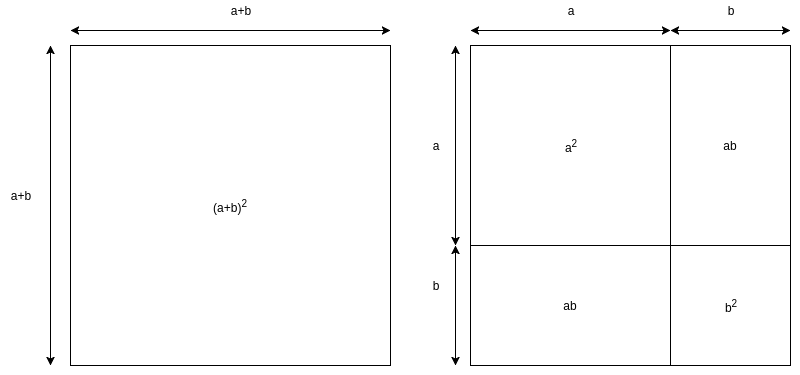
\includegraphics[width=\linewidth]{identity.png}
\caption{An Algebraic Identity Expressed Geometrically}
\label{fig:my_label19}
\end{figure}

Because the Greeks worked not primarily with individual number, but
instead \emph{magnitudes}: lengths, areas, volumes, and ratios thereof.
Because of this, algebraic identities such as
\[(a+b)^2 = a^2 + 2ab + b^2\] would have been expressed in terms of
relationships between geometric figures -- in this case, perhaps as
rearrangements of certain squares and rectangles, as
shown in the figure above.

Of primary interest to the Greeks was the solution of algebraic
equations by means of examining the intersection of algebraic curves. In
this way, they were led to study the \emph{conic sections}, those curves
which can be obtained by intersecting a plane with the surface of a
cone. In modern parlance, one might refer to such sections as those
traced out by real numbers \(x\) and \(y\) that satisfy a relationship
of the form \[Ax^2 +By^2 + Cxy + Dx + Ey + F = 0,\] where the
coefficients \(A\) through \(F\) are also taken to be real. Despite not
quite having the algebraic notation to state the problem in this form
nor the benefit of modern analytic and algebraic tools, the Greeks were
able to characterize all such sections, yielding circles, ellipses,
hyperbolas, parabolas, straight lines, and the degenerate case of a
single point.

\begin{figure}[H]
\centering
\begin{subfigure}[b]{0.3\textwidth}
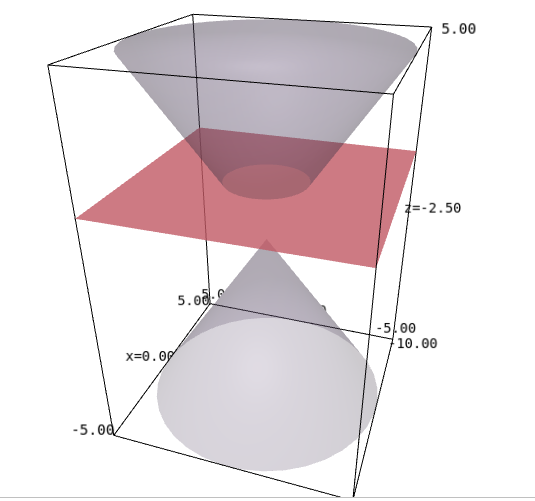
\includegraphics[width=\textwidth]{Selection_050}
\caption{A Circle}
\label{fig:gull21}
\end{subfigure}
~ %add desired spacing between images, e. g. ~, \quad, \qquad, \hfill etc.
%(or a blank line to force the subfigure onto a new line)
\begin{subfigure}[b]{0.3\textwidth}
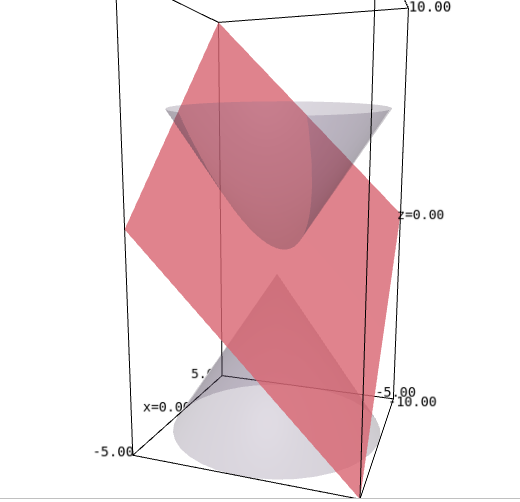
\includegraphics[width=\textwidth]{Selection_051}
\caption{A Parabola}
\label{fig:tiger23}
\end{subfigure}
~ %add desired spacing between images, e. g. ~, \quad, \qquad, \hfill etc.
%(or a blank line to force the subfigure onto a new line)
\begin{subfigure}[b]{0.3\textwidth}
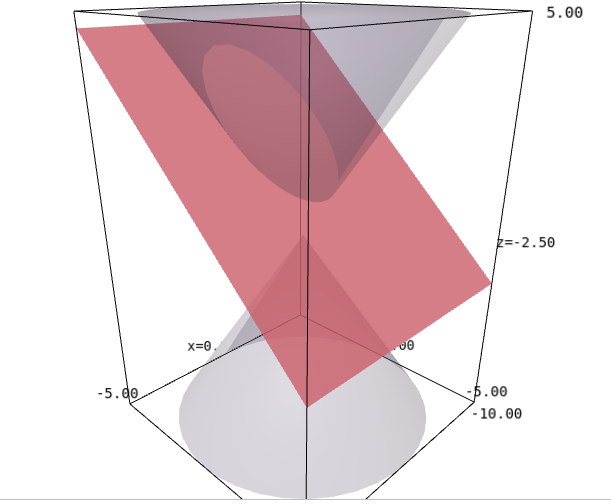
\includegraphics[width=\textwidth]{Selection_052}
\caption{An Ellipse}
\label{fig:mouse2}
\end{subfigure}

\begin{subfigure}[b]{0.3\textwidth}
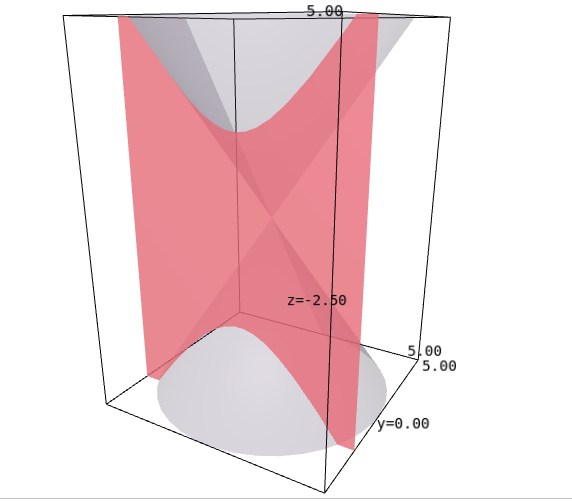
\includegraphics[width=\textwidth]{Selection_053}
\caption{A Hyperbola}
\label{fig:gull2}
\end{subfigure}
~ %add desired spacing between images, e. g. ~, \quad, \qquad, \hfill etc.
%(or a blank line to force the subfigure onto a new line)
\begin{subfigure}[b]{0.3\textwidth}
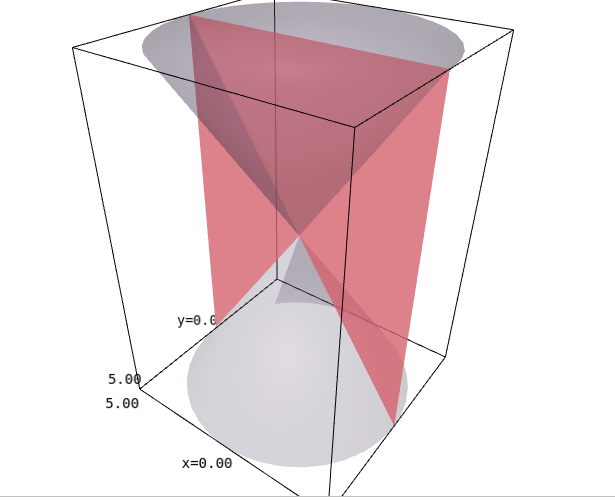
\includegraphics[width=\textwidth]{Selection_055}
\caption{Two Lines}
\label{fig:tiger3}
\end{subfigure}
~ %add desired spacing between images, e. g. ~, \quad, \qquad, \hfill etc.
%(or a blank line to force the subfigure onto a new line)
\begin{subfigure}[b]{0.3\textwidth}
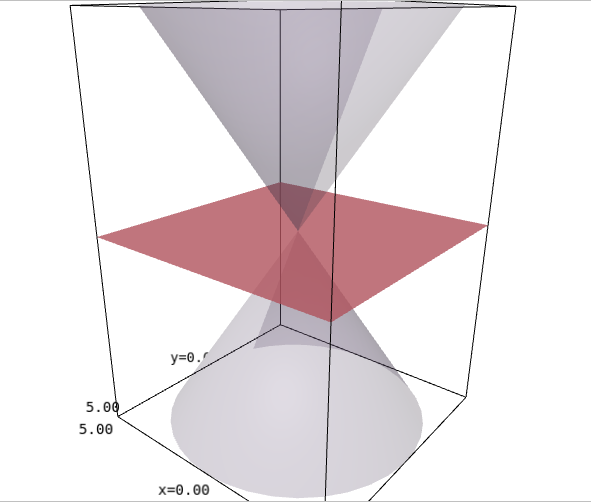
\includegraphics[width=\textwidth]{Selection_054}
\caption{A Single Point}
\label{fig:mouse4}
\end{subfigure}
\caption{The Conic Sections}\label{fig:animals27}
\end{figure}

Accordingly, the Greeks were aware of methods (for example) to solve
problems such as ``squaring the rectangle'', to which one might associate
equations of the form \(x^2 = ab\), regarding the quantity \(x^2\) as
the area of a unknown square and both \(a\) and \(b\) as known side
lengths. In their mathematical framework, all such constructions were
necessarily geometric in nature, and were thus restricted to those which
could be obtained with use of a compass and straightedge. In these
terms, such a problem might be cast as finding the solutions \(x\) that instead satisfy the cross-ratio \[\frac{x}{b} = \frac{a}{x}\]

A similar example is the problem of ''doubling the cube'' -- that is, given a cube
with known side lengths, constructing a second cube with exactly twice
the volume of the first. This amounts to finding \(x\) that satisfy a
similar ratio, \[\frac{x^3}{a^3} = \frac{b}{a}\] Considering the
simplest case of the unit cube led to questions concerning whether
number such as \(\sqrt[3]{2}\) were constructible in the geometric sense
described above, a question that would remain unsolved until the advent
of the algebraic tools of Galois Theory in the \nth{19} century.

However, although in many cases the Greeks made use of coordinates,
their study of geometry did not have the same analytic flavor that it
takes on today -- the modern notion of a coordinate system would not
enter the mathematical zeitgeist until nearly the \nth{17} century, with the
work of Rene Descartes. Moreover, the classical study was restricted to
algebraic curves in at most 3 dimensions, and usually over fields such
as $\RR$ or $\QQ$, and so it remained until the ``Geometric
Renaissance'' of the \nth{18} and \nth{19} centuries.

\subsection{Modern Times}\label{header-n42}

Due to reverence of the infamous fifth postulate of Euclid, the study of
\emph{synthetic geometry} -- that built on a collection axiomatic
foundations -- remained the dominant mode of Geometric thought. With the
advent of Cartesian coordinates, however, a separate study of
\emph{analytic} (or coordinate) geometry began, coinciding with the
beginning of the study of alternative geometries based upon negating the
fifth postulate. However, the unreasonable effectiveness of coordinates
in applications to science and engineering endeavors, along with the
invention of Calculus in the mid \nth{17} century, led to the flourishing of
the analytic branch in favor of synthetic approaches.

And so it remained until roughly the \nth{19} century -- it was at this point
in time that it began to become apparent that alternative and equally
valid non-Euclidean geometries could arise from the negation of the
fifth postulate, leading to the study of elliptic and hyperbolic
geometries. In particular, during this period there was a resurgence of
the field of \emph{projective geometry}, which was originally studied by
Brunelleschi as the ``geometry of perspective'' in the \nth{15} century, and
reformulated in terms of ``points at infinity'' around the \nth{17} century by
Kepler and Desargues.

Around this time, a notion of \emph{affine geometry} had also come into
the picture, which is roughly characterized as a generalization of
Euclidean geometry in which the notion of absolute distance is
forgotten, and the concepts that remain meaningful are instead the
notions of parallel lines, collinearity, and the preservation of certain
ratios. It was known early on that Euclidean geometry could be recovered
as a special case of projective geometry, and as affine geometry and new
non-Euclidean geometries were discovered, it was soon thought that
\emph{all} such geometries could in fact be recovered in such a way,
making projective geometry a more general and universal theory.

A major proponent of this point of view in the \nth{19} century was Felix
Klein (of Klein Bottle fame), who sought to classify all geometries with
his \emph{Erlangen Program}. He believed that projective geometry would
provide a unifying framework under which all other geometries could be
united, and introduced the idea that such geometries could be
characterized using the theory of groups. It was with the advent of
Klein's program that traditionally synthetic approaches found rigorous
footing in analytic and algebraic notions.

\section{The Erlangen Program}\label{header-n51}
\subsection{Euclidean Geometries}

In particular, the \textit{Erlangen} program laid out a framework in which any given
geometry could be categorized as a group of symmetries acting on a
vector space, and it is of some interest to see how such constructions can yield familiar geometries.

For example, fix some field \(k\) -- in the familiar setting, one might
choose \(\RR\), but many interesting ideas can be brought to light by considering the
general case. One can choose a coordinate system and consider sets of
ordered \(n\)-tuples
\[k^n \definedas \theset{(k_1, k_2, \cdots k_n) \mid k_i \in k}.\]
Equipping this set with the usual point-wise operations of addition and scalar
multiplication, a vector space \(V_k\) of \(n\)
dimensions over the base field \(k\) can be obtained. With a vector space in hand, one
can consider linear maps from \(V_k\) to itself (sometimes referred to as \textit{operators}), and if \(n\) is finite,
these are entirely characterized by \(n\times n\) square matrices. In
particular, one can form groups of such matrices by equipping them with the usual notion of matrix multiplication, and examine the
actions of these groups on \(V_k\).

Since several such groups will be useful in recovering
familiar geometries, a few definitions are in order. In each situation,
it will be assumed that \(k\) is a field, and \(V_k\) is a vector space
of finite dimension \(n\) over the field \(k\).

\begin{definition} The set of \(n\times m\) matrices with entries in \(k\) will
be denoted \(M_{n,m}(k)\). If \(n=m\), this will simply be abbreviated
to \(M_n(k)\), which denotes the set of \(n\times n\) (or \textit{square}) matrices over
\(k\).
\end{definition}

In general, a square matrix is equivalently a mapping from
\(V_k\) to itself, which can be realized via matrix-vector multiplication. One is often
interested in such mappings that are invertible, which prompts the next
definition.

\begin{definition} The \emph{general linear group of dimension \(n\),}
\(GL_n(K)\), is the group defined by the set
\[GL_n(K) \definedas \theset{M \in M_n(k) \mid \det (M) \neq 0},\] 
equipped with matrix multiplication. Equivalently, this is
the set of invertible
(and necessarily square) matrices with entries in \(k\).
\end{definition}

The general linear group can alternatively be characterized as a representation of the set of
invertible linear operators on \(V_k\), equipped with
function composition. For the purpose of this discussion, this group is
quite large, so we will be interested in certain subgroups.

\begin{definition} The \emph{orthogonal group of dimension \(n\)}, \(O_n(k)\),
is defined as the set \[O_n(k) \definedas \theset{M \in GL_n(k) \mid MM^T = I},\]
equipped with matrix multiplication, where
\(M^T\) denotes the transpose of a matrix and \(I\) denotes the unique $n\times n$ matrix that satisfies \(AI = IA = A\) for every
\(A\in M_n(K)\).
\end{definition}

It can be shown \(O_n(k)\) is in fact a subgroup of \(GL_n(k)\).
Equivalently, it can be characterized by those matrices \(M\) for which
\(M^{-1}\) = \(M^T\), or equivalently those for which \(\det M = \pm 1\). If
one takes \(k=\RR\), these are exactly the distance-preserving
transformations (often referred to as \emph{isometries}) of \(\RR^n\)
that preserve the origin. Taking the dimension to be either 2 or 3
reveals that this produces a group consisting of both rotations around
the origin, and reflections \emph{through} the origin.

In Euclidean geometry, one is also interested in translating and
transporting one figure to another point in space, which motivates the
next definition.

\begin{definition} The \emph{group of translations} in vector space \(V_k\) of
dimension \(n\) is denoted \(T_n(k)\), and is equivalent to \(k^n\), the
set of all \(n\)-tuples with entries in \(k\).
\end{definition}

The above definition is a consequence of the fact that any translation
can be identified with a vector along which the translation occurs,
which does not depend on the point being considered.

Equipped with these definitions, we can finally define one of the main
groups of interest that will help characterize Euclidean geometry:

\begin{definition} The \emph{Euclidean group of dimension n} is the group
defined by \(E_n(k) \definedas T_n(k) \rtimes O_n(k)\), the semi-direct
group product of the group of translations with the orthogonal group.
\end{definition}

The purpose of this definition is to capture some of what is already known about
Euclidean geometry -- it is invariant under rigid motions (or
isometries), which can, in turn, be characterized by combinations of
translations, rotations, and reflections about lines. It is
these exact types of motions that preserve the essential elements of
classical Euclidean geometry -- length, angle, ratios, parallel lines,
and intersections of lines.

While defining the notion of a semidirect product is perhaps outside the
scope of this paper, it happens to be the exact algebraic tool that
describes how such isometries can be constructed. In this case, it
captures the notion the if one first performs a translation, followed by
a rotation or reflection, this motion can equivalently be carried out by
first performing the rotation or reflection, and then translating by the
new rotated or reflected image of the original translation vector.

Taking a field such as \(\RR\) and the dimension of \(n=2\), we find
that the vector space \(\RR^2\) along with the group \(E_2(\RR)\)
provides enough information to recover classical Euclidean geometry in the plane.

\subsection{Affine Geometries}\label{header-n86}

In the affine case, one is often interested in maps
\(T: k^n \rightarrow k^n\) of the form \(v \mapsto Mv + b\) where \(M\)
is a linear translation and \(b\) is another vector in \(k^n\). These
maps are often called \emph{affine transformations}, and spaces that result from quotienting by this action are \textit{affine spaces}, which are often described as ``vector spaces in which the origin is
forgotten.'' Another way of stating this is that allowing the morphisms
to be combinations of both linear maps \emph{and} translations obviates the need for a
distinguished zero vector, and allows one to equivalently treat similar
figures without reference to an absolute coordinate system.

While this may seem like an abstract notion, it is, in fact, one that is
commonly and implicitly used by anyone who has worked with vector spaces
in any capacity: vector spaces are in fact affine spaces over
themselves. It is this fact that allows one to denote a \emph{vector} in
this space by an \(n\)-tuple of points, and to interchangeably use the same notation for
a \emph{point} of that space. Similarly, one commonly uses the affine
structure of a vector space when transporting a vector to a chosen
origin and treating it equivalently to the original vector.

Affine transformations are themselves more general than linear
transformations. For one, linear maps must preserve the origin, sending
zero to zero, while affine maps may not. In addition to the rotations
and translations present in the Euclidean case, elements of the affine
group additionally may induce both uniform and non-uniform scaling, as
well as shearing of figures. And in contrast to the Euclidean case,
affine transformations do not in general preserve angles and distances --
they do, however, still preserve straight lines, and send parallel lines
to parallel lines.

In order to obtain this type of geometry in the framework of the
Erlangen program, one can carry out similar constructions to arrive at
the following result:

\begin{definition} The \emph{affine group of dimension \(n\)} is defined as
\(Aff_n(k) \definedas T_n(k) \rtimes GL_n(k)\).
\end{definition}

As noted previously, the group \(O_n(k)\) is a subgroup of \(GL_n(k)\), and
so this result suggested to Klein and his contemporaries that Euclidean
geometry was, in fact, a restriction, or special case, of affine geometry.

\subsection{Projective Geometries}\label{header-n99}

In the case of projective geometry, one wants to introduce a notion of
``perspective projection'' in addition to the isometries obtained in the
Euclidean and Affine cases. However, in order to do so, one must forego
the preservation of parallel lines. This is a consequence of the early
study of the subject, with respect to capturing 3-dimensional images on
a 2-dimensional medium. This required the introduction of a point at
which all parallel lines in the image would meet, which is now referred
to as a \emph{vanishing point} or a \emph{point at infinity}.

\begin{figure}[h]
\centering
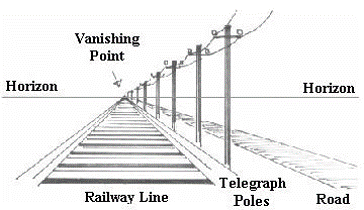
\includegraphics[width=0.8\linewidth]{vanishing.png}
\caption{Using a Vanishing Point for Perspective Projection}
\label{fig:my_label7}
\end{figure}

To see why Klein considered Projective geometry to be the
most general and universal among the geometries known at his time, it
suffices to carry out a similar construction in the projective case. One
first takes a vector space \(V_k\), constructs a group that will act as
the symmetries that preserve the desired properties, and identifies the geometry as the space that remains invariant under such a group action. In the projective case, the group itself is constructed in a slightly different way, and so a definition from group theory is needed.

\begin{definition} Given a group \(G\), the \emph{center} of a group \(Z(G)\)
is defined as
\(Z(G) \definedas \theset{g\in G \mid gh = hg ~\forall h\in G}\), the
set of elements that commute with every other element of the group.
\end{definition}

\begin{definition} The \emph{projective linear group of dimension \(n-1\)} is
the group defined by \(PGL_{n-1}(k) = GL_n(k) / Z(GL_n(k))\), the
general linear group quotiented by its center.
\end{definition}

The \(n+1\) condition is the first noticeable difference, which arises
from the fact that a projective space of dimension \(n\) is obtained
from a vector space of dimension \(n+1\), and the projective
transformations (often called \emph{homographies}) are induced by the
linear transformations in that vector space. Such projective
transformations play an important role in complex analysis, where one
can realize the \emph{Mobius group} \(PGL_2(\CC)\) as fractional linear
transformations on the Riemann sphere \(\CC \cup \theset{\infty}\),
which could equivalently be denoted the \emph{complex projective line}.

It can then be shown that, for fixed \(k\) and \(n\), both the Euclidean
and Affine groups are isomorphic to subgroups of the Projective group,
and it is in this way that those geometries can be recovered as special
cases of projective geometry.

\section{Into the \nth{20} Century}
\subsection{Post-Erlangen Program}\label{header-n112}

Armed with the tools of the Erlangen program, geometry once again become
an active mathematical research topic and its impact rippled
throughout the \nth{19} and \nth{20} centuries. It was one of the first moderately successful modern attempts
to provide a unifying framework under which many disparate parts of
mathematics could be connected and derived from one another, revealing
new connections and insights.

It is a fact that the program was not all-encompassing - for example,
the recently developed Riemannian geometry did not easily fit into
this framework. But perhaps its most significant and lasting impact on
Mathematics lies in its cultural effects, and in particular, in the way it affected how
mathematical knowledge was organized and synthesized. It proved the
usefulness of having such unifying frameworks, a theme that would become
prominent in the \nth{20} century, and laid the groundwork for the
philosophy that would drive the development of category theory in the 1940s.

\subsection{The Italian School}\label{header-n104}

Meanwhile, the field of Algebraic Geometry progressed
somewhat independently, but it became clear that affine and projective spaces were
fundamental to the subject, as were functions (and particularly
polynomials) on those spaces. Major work was done in this area in the late \nth{19} and early \nth{20} centuries by a group referred to as ``The Italian School'' in Rome, primarily driven by the work of Severi, Castelnuovo, and Enriques. In order to discuss the significance of their work, however, it is necessary to introduce several more definitions.

\begin{definition}
\emph{Affine \(n\)-space} over a field \(k\), denoted
\(A^n(k)\) is defined as the set of \(n\)-tuples
\((k_1, k_2, \cdots k_n)\), along with the information of the vector
spaces \(V_k\) of dimension \(n\) over \(k\) and the action of the
affine group \(Aff_n(k)\) on \(V_k\).
\end{definition}

In many ways, this is very similar to the vector space \(k^n\) defined
previously, and in fact, there is a map \(k^n \rightarrow A^n(k)\) that
is colloquially referred to as ``forgetting the origin'', and a reverse
map \(A^n(k) \rightarrow k^n\) that amounts to choosing a coordinate
system. An affine space is chosen generally when one doesn't need the
full structure of a vector space, but would still like to consider
notions such as points, relative distances, collinearity, and the other
isometries preserved by the affine group.

If one then fixes some multivariate polynomial \(p\) in the polynomial ring
\(k[x_1, x_2, \cdots, x_n]\) over \(n\) indeterminates with coefficients
in \(k\), one can examine points of the form
\[\bar{a} = (a_1, a_2, \cdots a_n)\] in \(A^n(k)\) such that
\(p(a_1, a_2, \cdots, a_n) = 0\). The collection of such points is
referred to as the \emph{zero locus} of such a polynomial, or
equivalently an \emph{algebraic hypersurface}.

For example, take \(k=\RR\) and consider polynomials of degree 2 in
\(k[x,y]\). In generality, the hypersurface of such a polynomial
\(p(x,y)\) will be defined by the relation
\[p(x,y) = Ax^2 + By^2 + Cxy + Dx + Ey + F = 0,\] where the coefficients
\(A-F\) are taken to be real numbers. But this exactly describes the
general equation of a conic section, as studied by the Greeks, and so we
find that this new notion of a hypersurface perfectly generalizes
algebraic surfaces such as conic sections, but allows for variation in
both dimension and base field.

This prompts the following definition:

\begin{definition}
Given a set \(S\subseteq k[x_1, x_2, \cdots x_n]\) of the
form \(S = \theset{p_1, p_2, \cdots p_m}\), the \emph{affine algebraic
variety of \(S\)} is defined as
\[V(S) \definedas \theset{\bar{a} \mid \bar{a} \in A^n(k), ~ p_i(\bar{a}) = 0~ \forall p_i \in S}.\]
(Note that the set \(S\) is sometimes referred to as a \emph{system} of
polynomials.)
\end{definition}

In other words, one can take a number of polynomials and consider the
points where they \emph{simultaneously} vanish, which is equivalent to
looking at the intersections of their associated hypersurfaces, and
combine all of this information into a structure called a
\emph{variety}. It is these objects -- roughly speaking, the zero loci
of polynomials -- that form one of the fundamental structures upon
which much Algebraic Geometry is based.

To see why such an object may be interesting, take \(k=\RR\), the ring
\(k[x,y]\), and consider the polynomial \[p_1(x,y) = y^2-x^3.\] The
variety \(V(\theset{p1})\) traces out an \emph{algebraic curve} in the
\(x\)-\(y\) plane, shown in the first figure below. In contrast, consider also the
polynomial \[p_2(x,y) = y^2-x^3+x,\] then \(V(\theset{p_2})\) is also an
algebraic curve, as shown in the second figure. Finally, consider
\[p_3(x,y) = y^{2} - x^{3}-3x^{2},\] shown in the third figure.

\begin{figure}[H]
\centering
\begin{subfigure}[b]{0.3\textwidth}
\includesvg[width=\textwidth]{cusp-point}
\caption{$y^2-x^3 = 0$}
\label{fig:gull13}
\end{subfigure}
~ %add desired spacing between images, e. g. ~, \quad, \qquad, \hfill etc.
%(or a blank line to force the subfigure onto a new line)
\begin{subfigure}[b]{0.3\textwidth}
\includesvg[width=\textwidth]{double-point}
\caption{$y^2-x^3+x = 0$}
\label{fig:tiger2}
\end{subfigure}
~ %add desired spacing between images, e. g. ~, \quad, \qquad, \hfill etc.
%(or a blank line to force the subfigure onto a new line)
\begin{subfigure}[b]{0.3\textwidth}
\includesvg[width=\textwidth]{nice}
\caption{$y^{2} - x^{3}-3x^{2} = 0$}
\label{fig:mouse15}
\end{subfigure}
\caption{Examples of Algebraic Curves}\label{fig:animals17}
\end{figure}

An immediate qualitative difference is that \(p_1\) has a ``cusp'' near 0,
where it may be unclear what the correct assignment of a tangent line
should be, while the second is ``smooth'' but also has a ``double point'' at
which there are two possible choices for a tangent line. The third, on
the other hand, does not seem to exhibit any such irregularities, and is in fact an \textit{elliptic curve}, an object with a
rich analytic and algebraic structure.

The types of irregularities present in $p1$ and $p2$ are in general referred to as \emph{singularities} of the curve,
and so
one might be inclined to wonder what causes such singularities to occur,
and if there are perhaps conditions on the polynomials themselves that
might guarantee that the curves generated contain no such singularities.

Such questions drove many results in the classification of algebraic
curves and it was found that the \emph{genus} associated to the curve, an essentially topological property, was a powerful tool in such classifications. It was the extension of these ideas to the classification algebraic \emph{surfaces} in higher dimensions that the
Italian school focused their efforts on. To this end, many results were
produced, but their results and methods of proof have remained
contentious throughout the \nth{20} century.

\subsection{The Weil Conjectures and Grothendieck}\label{header-n127}

Various progress in other areas of geometry was made throughout the
first half of the \nth{20} century, most notably the advances of Hilbert and
his proof of the \emph{Nullstellensatz} (roughly translated as ``theorem
of zero loci''). Recalling that a variety was defined over system \(S\)
of polynomials, where \(S\) is contained in some polynomial ring
\(k[x_1, x_2, \cdots, x_n]\), one form of the \emph{Nullstellensatz}
shows that if one wants to check whether the variety \(V(S)\) is
nonempty, one can equivalently check whether \(S\) is a (proper) ideal
in this ring. This firmly cemented the link between Algebra and
Geometry, providing a bridge that allowed many of the tools from either
one of these fields to be used in the other.

Around 1950, a mathematician named Andre Weil set forth ``The Weil
Conjectures'', three proposals that stem from setting \(k\) to be a
finite field, considering the resulting varieties, and defining analogs
of the Riemann-Zeta function in order to count the number of rational
points on the resulting algebraic curves. Weil conjectured that certain
properties similar to the traditional Zeta function should hold,
particularly with respect to the locations of their zeros.

In doing so, he was able to formulate an analog of the Riemann
Hypothesis for these situations, and further conjectured that many of the
newly formed tools of homological algebra could be brought to bear on
such a problem. Homological tools had proved to be both powerful and
successful in topology in the first half of the century, and it was at
this point that many researchers were beginning to generalize such
theories and apply them to other areas. In particular, Weil suspected
that applying homological methods from algebraic topology to these
conjectures would have significant number-theoretic ramifications.

It is here that Alexandre Grothendieck enters the picture, as well as
his contemporary John-Pierre Serre, for within 15 years Grothendieck had
published solutions to two out of three of these conjectures. In the process, he introduced many of the tools that would become standard in modern Algebraic Geometry -- his major contributions being in the development of the necessary homological tools, a cohomology theory for varieties. Such contributions were framed within the recently developed language of category theory, and included the definitions of abelian categories, derived functors, injective resolutions, schemes, and sheaves.

Grothendieck's general approach, which has gained traction widely across
mathematics in the resulting years, was noticing that certain classes of
geometric objects could be characterized by instead considering all of
the maps \emph{into} that object from other similar objects. In
particular, this applies to algebraic variety -- one can associate to a
given variety a collection of particularly well-behaved functions on
that variety, the so-called ``regular'' functions, and in this way study
the variety itself.

This collection of functions constitutes the simplest example of a
\emph{sheaf}, modulo a number of technical conditions. Perhaps more surprisingly, this collection forms a ring.
Given any ring \(R\), one can form the set of prime ideals of \(R\),
denoted \(\text{Spec}(R)\), and even equip with with a topology (what is
usually referred to as the \emph{Zariski topology}. If one then
introduces a topological space into the picture, there is a construction
entitled the \emph{structure sheaf} on the space which contains
information about the functions on that space, and taking a topological
space along with such a structure sheaf produces what is known
as a \emph{scheme}.

Although the construction of scheme itself is quite a bit more detailed and nuanced than what has been described here, its power lies
in its similarity to notions in differential geometry, where homological
methods had been successfully applied prior to Grothendieck. It is in this way that many
powerful tools from the study of manifolds can be generalized to work on
algebraic objects, and similarly to allow advances in the algebraic
theory of rings to be brought to bear on geometric problems.

However, such constructions proved to not just be limited to making connections
between geometry, topology, and algebra, but as Weil had hoped, laid the
groundwork for many of these tools to be applied to number theory. This
culminated in the celebrated proof of Fermat's Last Theorem by Andrew
Wiles in the 1990s, which built upon on many of the tools developed
during this period.

\section{Conclusion}

In summary, perhaps the most notable influence of Algebraic Geometry on
the face of mathematics has been the bridges it has created between
different fields. In its study, many mathematical ``Rosetta Stones'' have
been built, allowing deeper connections to be built between seemingly disparate
fields of mathematics, and moreover making possible the transport of
powerful techniques across these domains. In the latter half
of the \nth{20} century, Grothendieck left the world of Mathematics,
and spent most of his remaining days in solitude, living in the Pyrenees until his death in 2014. And although mathematics is not a lone
endeavor, it is particularly hard to overstate the singular
contributions of Grothendieck, for his ideas continue to shape how modern mathematics is formulated.

\newpage

\begin{thebibliography}{20}

\bibitem{goodgeometries}
Sosinskii, A. B. (2012). Geometries. Providence, RI: American Mathematical Society.

\bibitem{thebook}
Hartshorne, R. (2010). Algebraic Geometry. New York: Springer.

\bibitem{klein}
Klein, F. (1893). A comparative review of recent researches in geometry. (Programme on entering the philosophical faculty and the senate of the University of Erlangen in 1872). New York.

\bibitem{rudiments}
States, U. (1963). Rudiments of Algebraic Geometry. New York: Oxford University Press.

\bibitem{history}
Dieudonne, J. (1985). History of algebraic geometry: an outline of the history and development of algebraic geometry. New York: Chapman and Hall.

\bibitem{ideasofspace}
Gray, J. (2003). Ideas of space: Euclidean, non-Euclidean, and relativistic. Oxford: Clarendon Press.

\bibitem{undergrad}
Reid, M. (1990). Undergraduate Algebraic Geometry. Cambridge University Presss.

\bibitem{amsmonthly}
Mclarty, C. (2016). How Grothendieck Simplified Algebraic Geometry. Notices of the American Mathematical Society, 63(03), 256–265. doi:10.1090/noti1338

\end{thebibliography}

\end{document}